\documentclass[10pt,twocolumn,letterpaper]{article}

\usepackage{cvpr}
\usepackage{times}
\usepackage{epsfig}
\usepackage{graphicx}
\usepackage{amsmath}
\usepackage{amssymb}
\usepackage{booktabs}

% Include other packages here, before hyperref.

% If you comment hyperref and then uncomment it, you should delete
% egpaper.aux before re-running latex.  (Or just hit 'q' on the first latex
% run, let it finish, and you should be clear).
\usepackage[pagebackref=true,breaklinks=true,letterpaper=true,colorlinks,bookmarks=false]{hyperref}

% \cvprfinalcopy % *** Uncomment this line for the final submission

\def\cvprPaperID{****} % *** Enter the CVPR Paper ID here
\def\httilde{\mbox{\tt\raisebox{-.5ex}{\symbol{126}}}}

% Pages are numbered in submission mode, and unnumbered in camera-ready
\ifcvprfinal\pagestyle{empty}\fi
\begin{document}

%%%%%%%%% TITLE
\title{Writing News Captions with Bags of Attention}

\author{Alasdair Tran, Alexander Matthews, Lexing Xie\\
Australian National University\\
{\tt\small \{alasdair.tran,alex.matthews,lexing.xie\}@anu.edu.au}
% For a paper whose authors are all at the same institution,
% omit the following lines up until the closing ``}''.
% Additional authors and addresses can be added with ``\and'',
% just like the second author.
% To save space, use either the email address or home page, not both
}

\maketitle
%\thispagestyle{empty}

%%%%%%%%% ABSTRACT
\begin{abstract}
   In this work, we present an end-to-end captioning system for news articles
   that can handle entity names and out-of-vocabulary words. Our model achieves
   state-of-the-art results on the existing ``GoodNews" dataset. We also
   re-collected news articles from the New York Times, which are cleaner and
   more complete. This dataset allows us to explore approaches involving
   image positions. The code will be made available on GitHub.
\end{abstract}

%%%%%%%%% BODY TEXT
\section{Introduction}

Our main contributions are as follows:

\begin{itemize}
   \item We show that combining article attention with pre-trained contextualized
   word piece embeddings allows our model to generate captions containing
   relevant words that were not seen during training.

   \item We demonstrate that the location of the image within the article is an
   important signal for generating relevant news captions.

   \item We build on the “Good News” dataset to produce a larger and more complete
   news captioning dataset consisting of * articles from the New York Times and
   their 794K images with captions. In contrast to “Good News” our dataset
   contains the full article text, and the location of the image within the
   page.
\end{itemize}


\section{Related Works}

Recent image captioning systems are based mostly on ``Show, Attend, Tell"
\cite{Xu2015ShowAA}, which uses a simple hard attention over the image. Later
improvements include giving the model the option to not attend to any image
region \cite{Lu2016KnowingWT}, using reinforcement learning to directly
optimize for the CIDEr metric \cite{Rennie2016SelfCriticalST}, and using a
bottom-up approach to propose a region to attend to
\cite{Anderson2017BottomUpAT}. All of these system generate generic captions.

A more challenging task is to generate captions for news images, in which we
need to be able to generate entity names. There are non-neural approaches
\cite{Feng2013AutomaticCG,Tariq2017ACE}. Neural approaches include using the
word2vec representation of the article and and the VGG19 representation of the
image as context to the LSTM generator \cite{Ramisa2016BreakingNewsAA}.

Biten \etal~\cite{Biten2019GoodNews} further refined this approach by
developing a two-stage architecture to handle entity names. In the first stage,
the model generates a template with placeholders such as PERSON and
ORGANIZATION. In the second stage, the model finds the best matched sentence in
the article and replace the placeholder with an entity mentioned in that
sentence. They also created the ``GoodNews" dataset, which contains more
samples than MSCOCO \cite{Lin2014MicrosoftCC} and BreakingNews
\cite{Ramisa2016BreakingNewsAA} datasets.

\begin{figure}[t]
   \begin{center}
   \fbox{\rule{0pt}{2in} \rule{0.9\linewidth}{0pt}}
      %\includegraphics[width=0.8\linewidth]{egfigure.eps}
   \end{center}
      \caption{An example caption.}
   \label{fig:long}
   \label{fig:onecol}
   \end{figure}

\section{Dataset}

A summary of the original GoodNews dataset and our new dataset is shown in
Table \ref{tab:datasets}. The GoodNews+ dataset is our attempt at recollecting
the original GoodNews dataset. We managed to crawl all the original articles,
but the number of images is slightly less, either due to dead links or
not crawling images unrelated to the main article. GoodNews+ allows us to make the
following observations about the original GoodNews dataset:

\begin{itemize}
   \item On average, half of the article body is missing. This includes
         the first few paragraphs that might contain important information
         about the top caption.
   \item The dataset contains a small number Spanish articles.
   \item Sometimes images from the recommendation sidebar, which are not part
         of the main article, are included in the dataset.
\end{itemize}

This motivates us to recollect data from the New York Times in a more careful
manner. We call this NYTimes+.

\begin{table}[t]
	\caption {Summary of datasets}
	\label{tab:datasets}
	\centering
	\begin{tabular}{llll}
		\toprule
		  & GoodNews  & GoodNews+ &   NYTimes+ \\
		\midrule
      No of articles & 241 808 & 241 808 & 445 828 \\
      No of images   & 462 642 & 440 112 & 794 085 \\
      Article length & 451 & 963 & 974 \\
      Caption length & 18 & 18 & 18 \\
      Start month & Jan 10 & Jan 10 & Mar 05\\
      End month & Jul 18 & Jul 18 & Sep 19 \\
		\bottomrule
	\end{tabular}
\end{table}

In addition to having a more complete coverage, we also collect information
about the image position in each article. As shown in Figure \ref{fig:dist},
about 40\% of the articles have two or more images.

\begin{figure}[h]
   \begin{center}
   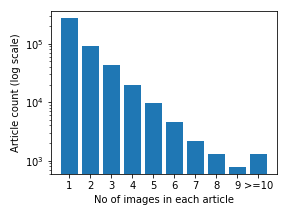
\includegraphics[width=0.8\linewidth]{figures/caption_dist.png}
   \end{center}
      \caption{Distribution of images across articles.}
   \label{fig:dist}
   \end{figure}




\section{Model}

Devlin \etal \cite{Devlin2019BERT} introduced BERT, a language representation
model which provides pretrained contextual embeddings for text. We use
RoBERTa \cite{Liu2019RoBERTaAR}, a more carefully trained BERT model, to
embed the article text. There there two key advantages:

\begin{itemize}
   \item Unlike glove \cite{Pennington2014Glove} or word2vec
   \cite{Mikolov2013DistributedRO} where each word has exactly one
   representation, the bidirectional and attention mechanism in transformers
   allow words to have different representation depending on the context.
   \item RoBERTa uses Byte-Pair Encoding (BPE)
   \cite{Sennrich2015NeuralMT,Radford2019LanguageMA} which allows us to
   represent and generate potentially any word that can be written in
   Unicode. The vocabulary size is 50,265.
\end{itemize}

Our decoder is a transformer architecture with dynamic convolutions
\cite{Wu2018PayLA} containing four layers with kernel sizes 3, 7, 15 and 31. We
found that using dynamic convolutions allows the training to converge faster
than using the current state-of-the-art GPT-2 architecture
\cite{Radford2019LanguageMA}. We don't have the computational resource to study
the performance of GPT-2.

To make training more efficient, we use adaptive softmax
\cite{Grave2016EfficientSA} and divide the vocabulary into three clusters: 5K,
15K, and 25K. We tie the adaptive weights and we share the decoder input and
output embeddings. We use sinusoidal positional encoding
\cite{Vaswani2017AttentionIA} to represent the position of each token.

We use ResNeXt-101 \cite{Xie2016AggregatedRT} to obtain an embedding for
the images. For each generation step, we use the Scalar-Dot-Product attention
\cite{Vaswani2017AttentionIA} to attend to the image and to article separate.
The two attended representations are then concatenated and fed as input to
the self-attention layer.

\begin{figure*}[t]
   \begin{center}
   \fbox{\rule{0pt}{2in} \rule{.9\linewidth}{0pt}}
   \end{center}
      \caption{Overall architecture of the model.}
   \label{fig:short}
   \end{figure*}

\section{Results}

Table \ref{tab:results-goodnews} shows the results on the original GoodNews
dataset. Table \ref{tab:results-nytimes} shows additional results done on
our NYTimes+ dataset.


\begin{table*}[t]
	\caption {Results on the GoodNews dataset}
	\label{tab:results-goodnews}
	\centering
	\begin{tabular}{llllllll}
		\toprule
		  & BLEU-1  & BLEU-2 & BLEU-3 & BLEU-4 & ROUGE & METEOR & CIDEr\\
		\midrule
      Biten \etal \cite{Biten2019GoodNews} & 8.92\% & 3.54\% & 1.60\% & 0.83\% & 12.1\% & 4.34\% & 12.8\% \\
      Transformer & 22.6\% & 13.7\% & 8.90\% & 6.15\% & 21.4\% & 10.3\% & 53.3\% \\
      \\
		\bottomrule
	\end{tabular}
\end{table*}

\begin{table*}[t]
	\caption {Results on the NYTimes+ test set}
	\label{tab:results-nytimes}
	\centering
	\begin{tabular}{llllllll}
		\toprule
		  & BLEU-1  & BLEU-2 & BLEU-3 & BLEU-4 & ROUGE & METEOR & CIDEr \\
		\midrule
      Transformer & 17.2\% & 10.2\% & 6.55\% & 4.55\% & 19.1\% & 8.41\% & 40.4\% \\
      Transformer (location-aware) & 18.4\% & 11.2\% & 7.35\% & 5.16\% & 20.5\% & 9.21\% & 47.6\% \\
      \\
		\bottomrule
	\end{tabular}
\end{table*}

\begin{table*}[t]
	\caption {Proper name metrics on the NYTimes+ test set}
	\label{tab:results-names}
	\centering
	\begin{tabular}{lllllll}
		\toprule
        & \multicolumn{2}{c}{All names} & \multicolumn{2}{c}{Rare names in caption } & \multicolumn{2}{c}{Rare names in article } \\
        & Recall  & Precision & Recall  & Precision & Recall  & Precision \\
		\midrule
      Transformer & 26.2\% & 31.5\% & 19.6\% & 29.3\% & 17.2\% & 21.3\%  \\
      Transformer (location-aware) & 30.1\% & 35.4\% & 23.6\% & 32.6\% & 22.1\% & 25.4\%   \\
		\bottomrule
	\end{tabular}
\end{table*}

\begin{table*}[t]
	\caption {Word statistics on the NYTimes+ test set}
	\label{tab:results-stats}
	\centering
	\begin{tabular}{lllllll}
		\toprule
        & Caption length  & Unique words \\
      \midrule
      Ground Truths & 18.4 & 17.1 \\
      Transformer  & 12.8 & 11.5 \\
      Transformer (location-aware) & 12.9 & 11.6  \\
		\bottomrule
	\end{tabular}
\end{table*}

\section{Conclusion}

{\small
\bibliographystyle{ieee_fullname}
\bibliography{paper}
}

\end{document}
